\apendice{Documentación de usuario}

\section{Introducción}
En esta sección se va a desarrollar el uso que se puede hacer de la aplicación por parte del usuario.
Este proyecto se compone de dos partes, un ejecutable y el servidor. 

\section{Requisitos de usuarios}

Este proyecto en el estado en el que se encuentra ahora se necesita arrancar el servidor en la máquina localmente pero en líneas futuras, esto no sería necesario para el usuario ya que está preparado para ser alojado en un servidor externo.

A continuación se van a presentar los requisitos que se necesita por parte del usuario: 
\begin{itemize}
    \item \textbf{Sistema operativo}: Debe de tener un sistema operativo Windows 10 o superior o Linux Ubuntu 18.04 o superior
    \item \textbf{Procesador}: Intel Core i3 o equivalente
    \item \textbf{Memoria RAM}: 4GB
    \item \textbf{Espacio en el disco}: Al menos 64GB de espacio libre
\end{itemize}

\section{Instalación}

Para poder ejecutar el proyecto en el dispositivo, se necesita instalar el Docker para poder arrancar el servidor en local. El proceso de instalación es igual a lo mencionado anteriormente en el manual del programador.
Se necesita descargar el repositorio de la siguiente url \url{https://github.com/etc99/algoritmosYmazmorras}.

\section{Manual del usuario}

\subsection{Manual del servidor}

Para poder visualizar los laberintos en el juego, primero es necesario tener arrancado el servidor. 
Para realizarlo es necesario abrir la terminal. 

En la terminal, con la ruta del directorio apuntando a \texttt{/Mamzmorras} se necesita ejecutar el siguiente comando para levantar el servidor:
\begin{lstlisting}
    docker compose up
\end{lstlisting}

Para poder parar el contenedor del juego, desde el teclado se pulsarían los botones Ctrl+C y para borrar el contenedor se realiza con el siguiente comando:
\begin{lstlisting}
    docker compose down
\end{lstlisting}

\subsection{Manual del juego}
Teniendo ya listo el servidor, ahora solo queda lanzar el ejecutable del videojuego. En la carpeta del ejecutable aparecerán diversos archivos, pero el ejecutable es el que se encuentra marcado en la figura \ref{fig:EjecutableUnity}.

\begin{figure}[!h]  
    \centering  
    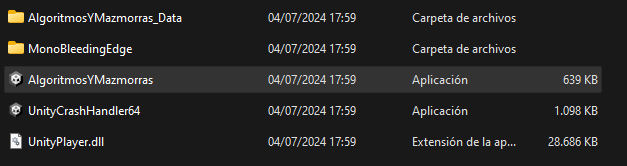
\includegraphics[width=\textwidth]{img/EjecutableUnity.png}  
    \caption{Carpeta del ejecutable de Unity.}  
    \label{fig:EjecutableUnity}
\end{figure}

Tras esto la primera pantalla que se mostrará es el menú principal como se muestra en la figura \ref{fig:MenuPrincipal}. Para poder avanzar a la siguiente pantalla se necesita pulsar sobre el botón de <<¡Comenzar!>>, al hacerlo se muestra la pantalla de selección de algoritmo \ref{fig:MenuSeleccion}.

Tras seleccionar uno de los algoritmos en la siguiente se mostrará lo que va a ser el tablero y el jugador, y en el margen izquierdo aparecerá un menú en el que se podrán introducir los parámetros deseados para el laberinto \ref{fig:ParametrosLaberinto}.

Después de introducir los parámetros se pulsa sobre el botón de <<Generar>>. Tras realizar esto se muestra el resultado para poder navegar el laberinto con las teclas <<W, A, S, D>> \ref{fig:LaberintoGenerado}.


\begin{figure}[!h]  
    \centering  
    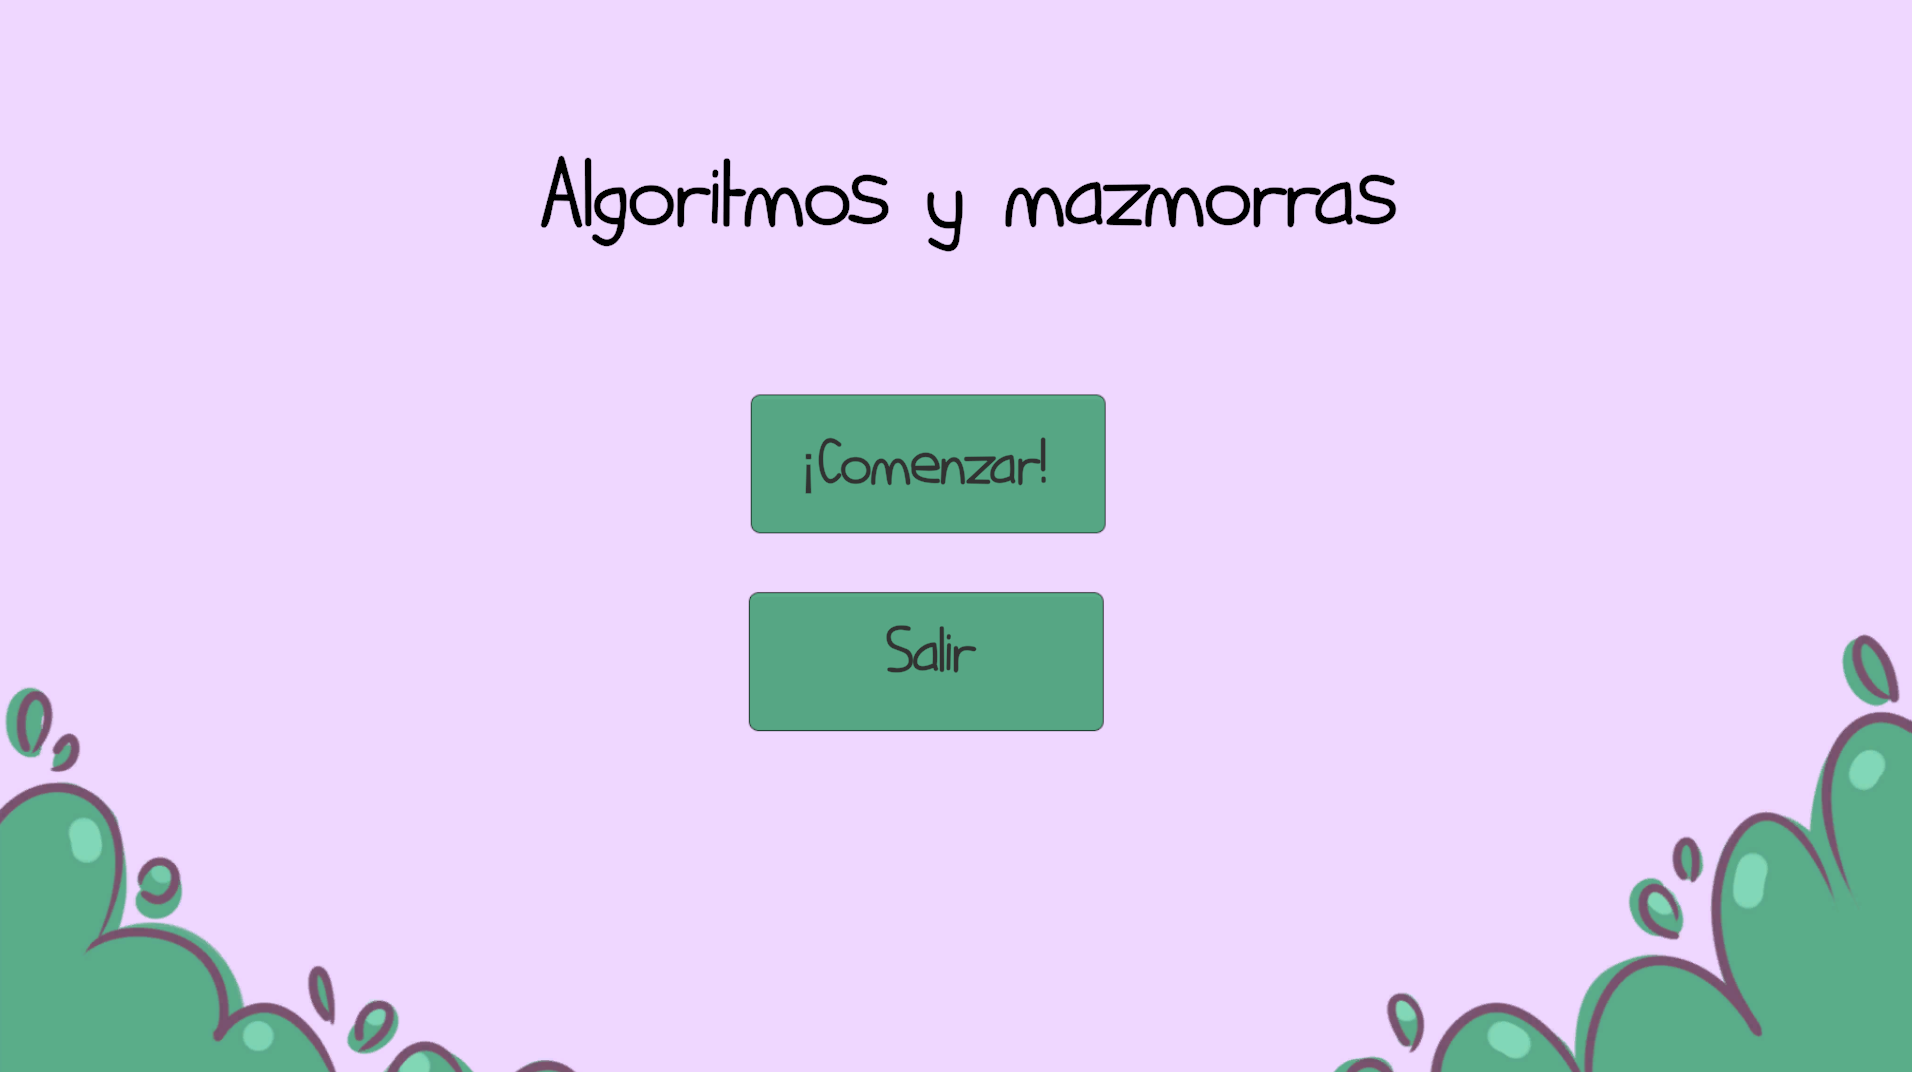
\includegraphics[width=\textwidth]{img/MenuPrincipal.png}  
    \caption{Captura del menú principal del juego.}  
    \label{fig:MenuPrincipal}
\end{figure}

\begin{figure}[!h]  
    \centering  
    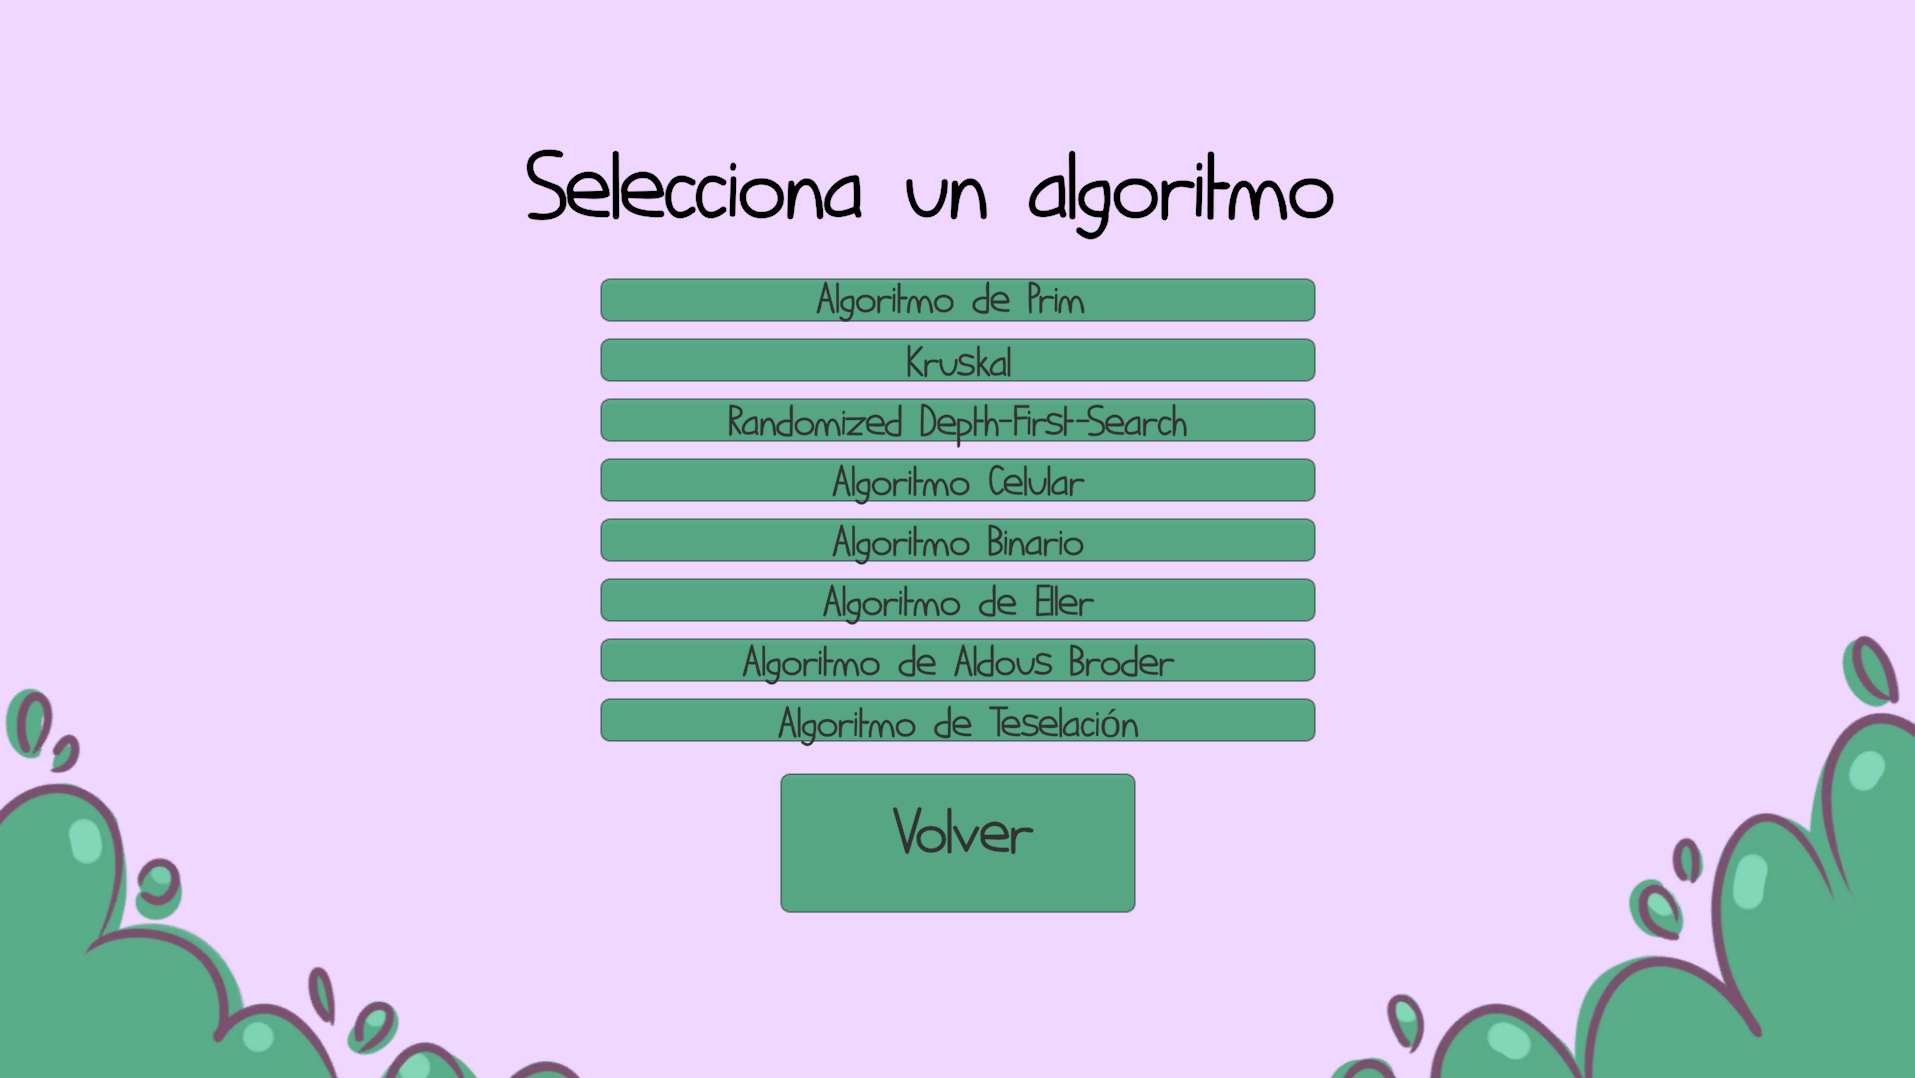
\includegraphics[width=\textwidth]{img/MenuSeleccion.png}  
    \caption{Captura del menú de selección de algoritmo.}  
    \label{fig:MenuSeleccion}
\end{figure}

\begin{figure}[!h]  
    \centering  
    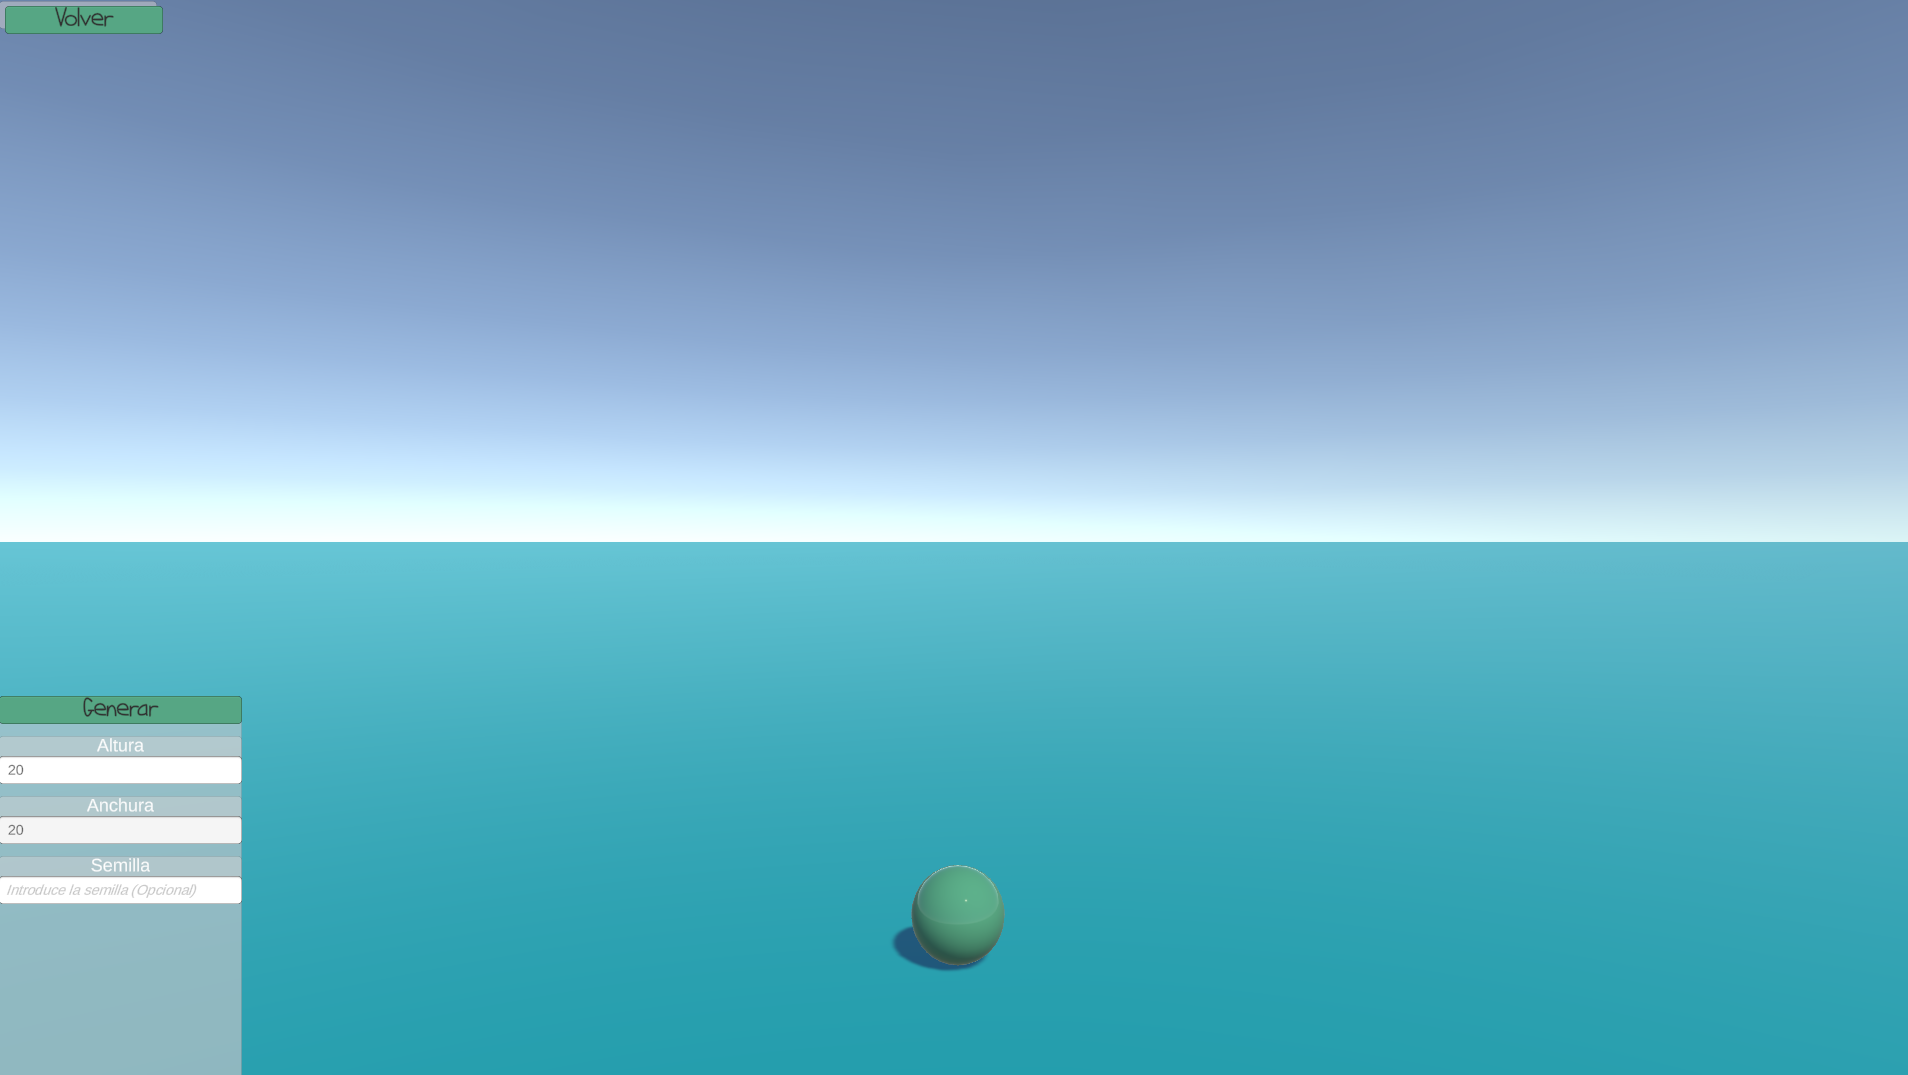
\includegraphics[width=\textwidth]{img/IntroducirParametrosLaberinto.png}  
    \caption{Captura de la interfaz para introducir los parámetros del laberinto.}  
    \label{fig:ParametrosLaberinto}
\end{figure}

\begin{figure}[!h]  
    \centering  
    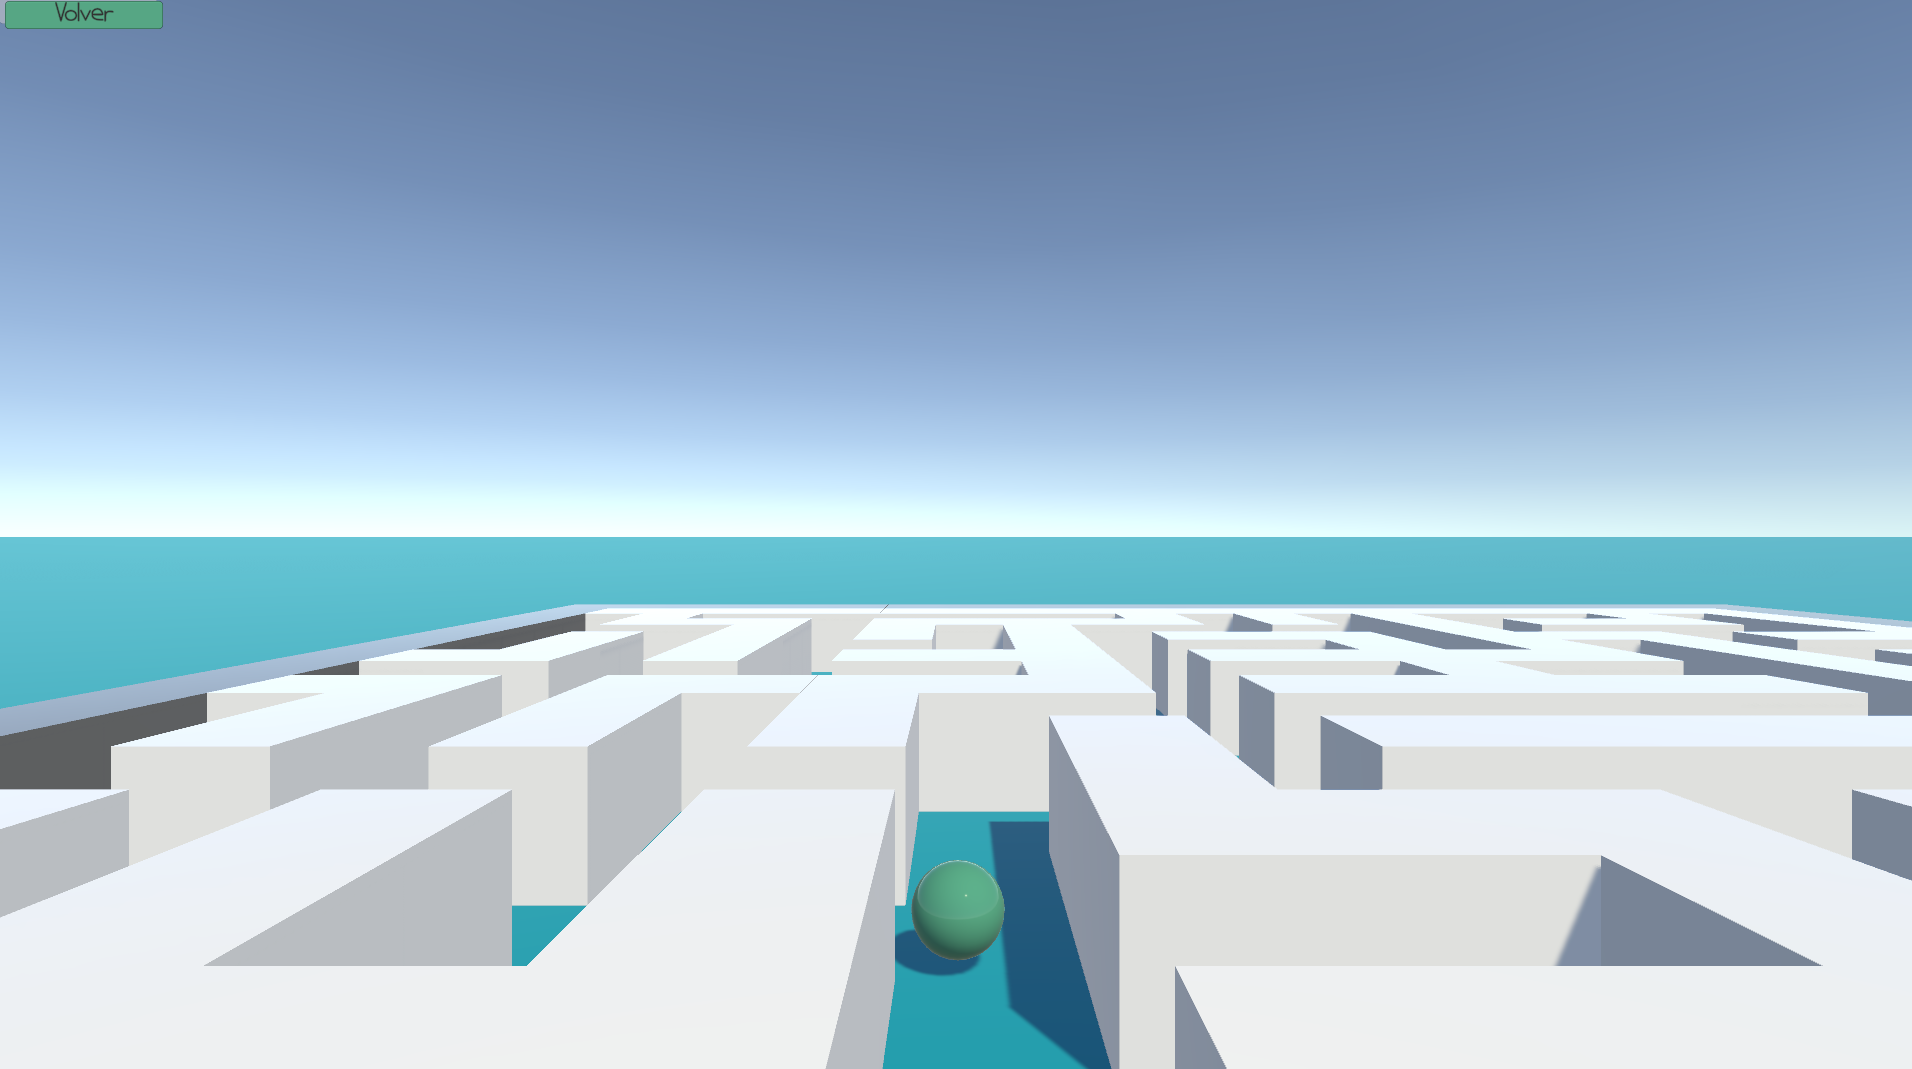
\includegraphics[width=\textwidth]{img/LaberintoGenerado.png}  
    \caption{Captura del laberinto generado.}  
    \label{fig:LaberintoGenerado}
\end{figure}